\subsection{EfficientPS}

EfficientPS é uma solução para a segmentação panóptica proposta no artigo \citeonline{mohan2020efficientps}, o trabalho apresenta uma arquitetura que se inicia com um backbone — parte para identificar características — usando uma FPN de 2 caminhos seguido de dois cabeçotes paralelos um para uma arquitetura de segmentação semântica que é autoria deles e outra de instância com modificações baseadas na topologia Mask R-CNN e finalmente a saída dos dois cabeçotes são combinadas no môdulo de fusão panóptica para gerar a saída final com a imagem de segmentação panóptica, esta arquitetura é ilustrada na \cref{fig:arqEP}.

\begin{figure}[H]
	\caption{Arquitetura geral do EfficientPS}
	\centering % para centralizarmos a figura
	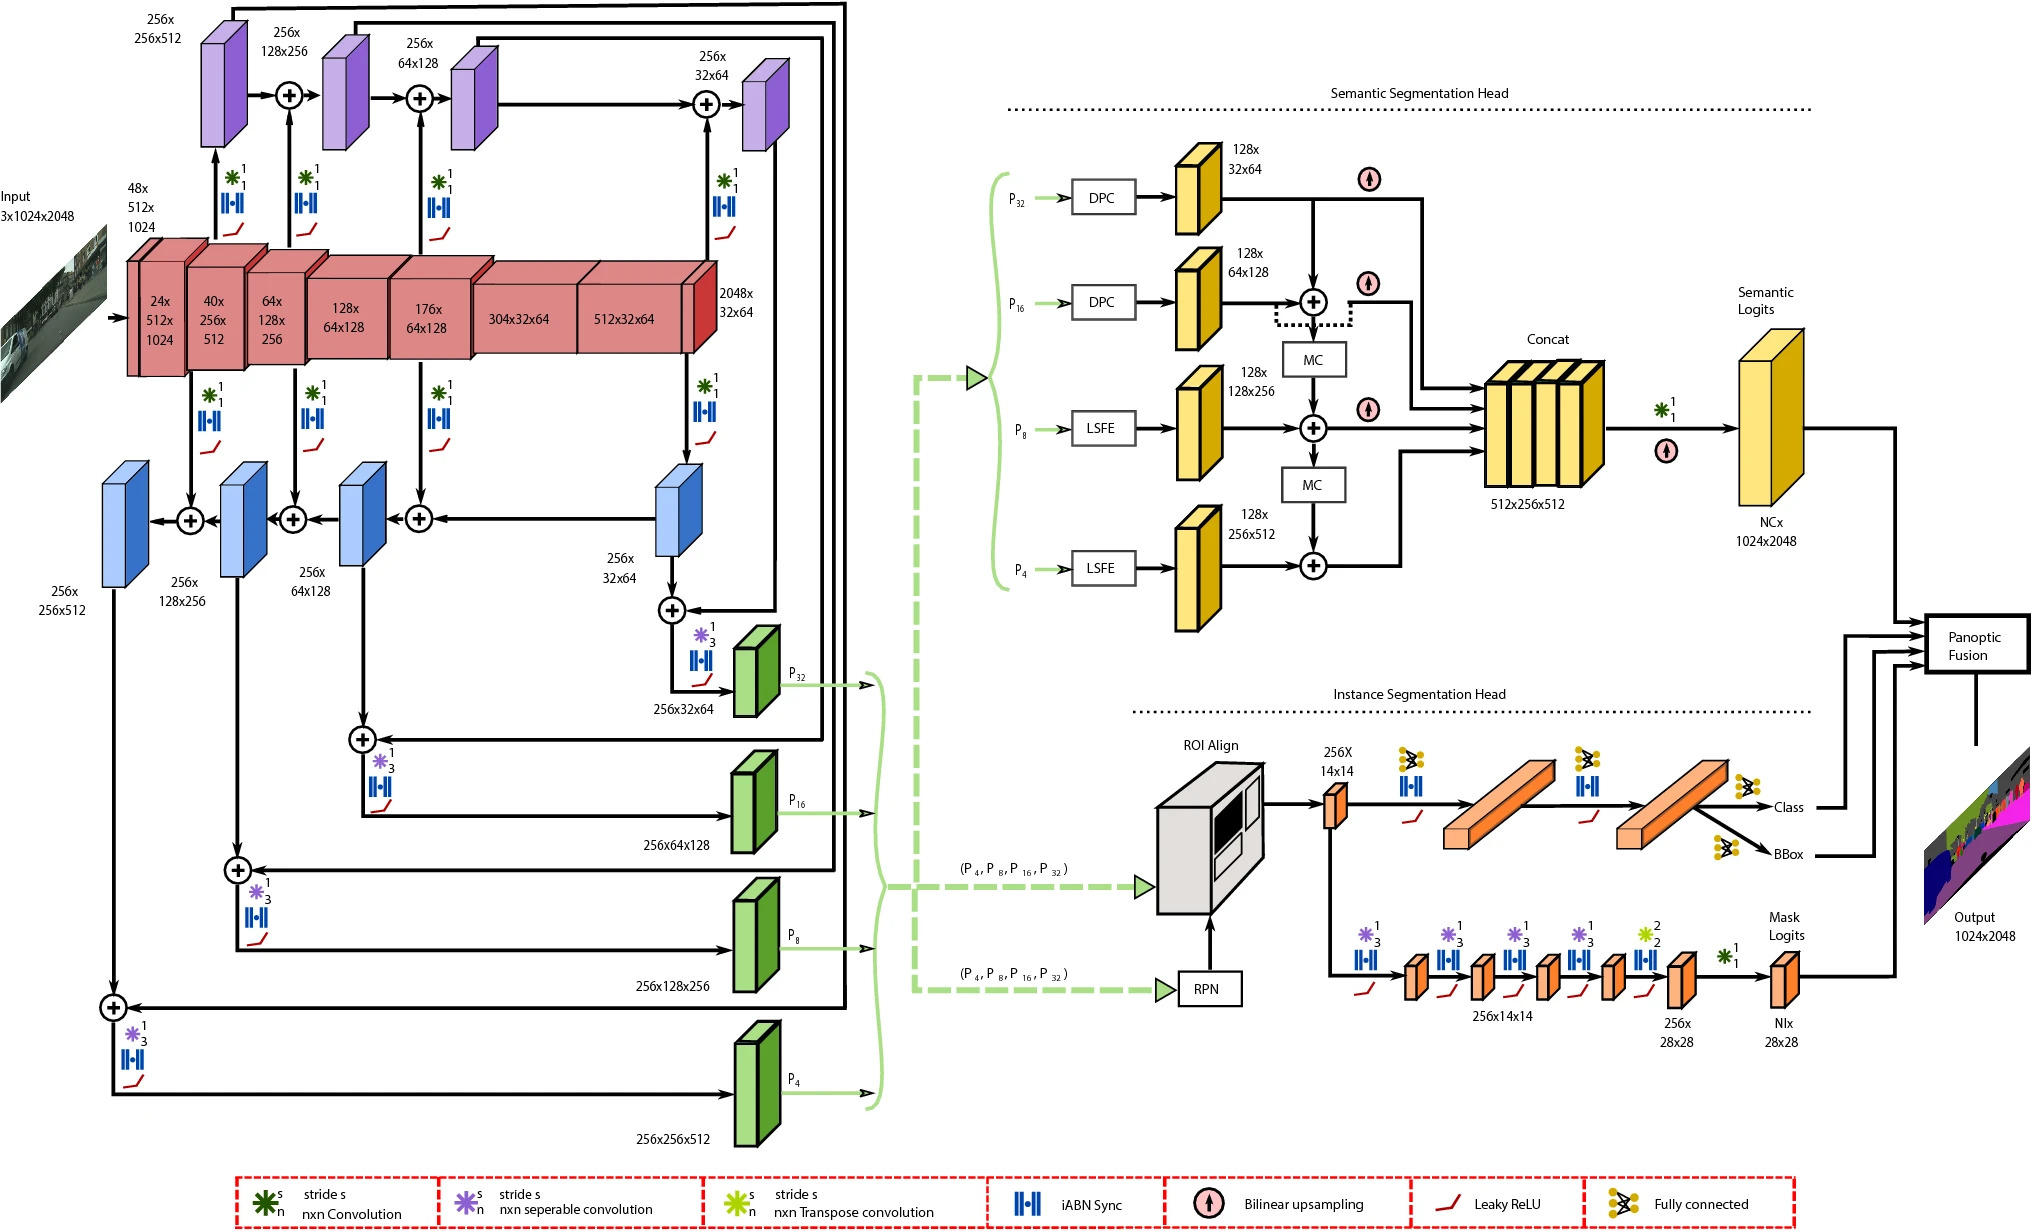
\includegraphics[width=15cm]{figures/arqEP.jpg} % leia abaixo
	\legend{Fonte: \citeonline{mohan2020efficientps}}
	\label{fig:arqEP}
\end{figure}

\subsubsection*{Backbone da rede}
A espinha dorsal — ou backbone — se consiste em uma codificação combinado a uma bifurcação paralela usando FPN. O codificador é essencial para arquiteturas de segmentação e para melhorar a capacidade de representação é necessário aumentar o número de parâmetros e a complexidade, porém nesse artigo os autores chegaram numa solução balanceada nesse quesito. O codificador contém nove blocos (em vermelho), mostrado na \cref{fig:arqEP} e a 2º, 3º, 5º e 9º saídas — da esquerda para diretira — correspondem aos fatores de redução de amostragem x4,x8,x16 e x32 respectivamente.


batch normalization
synchronized Inplace Activated Batch Normalization

\subsubsection*{Cabeçote de Segmentação Semântica}
O cabeçote de segmentação semântica é dividido em três môdulos sendo eles: extrator de características em larga escala — ou Large Scale Feature Extractor (LSFE) — para capturar recursos finos em larga escala de forma eficiente, módulo DPC deve ser capaz de capturar contexto de longo alcance porém em pequena escala e o módulo MC deve ser capaz de mitigar a incompatibilidade entre recursos de grande e pequena escala nas camadas de agregação.

As quatro entradas do cabeçote — $ P_4 + P_8 + P_16 + P_32 $ — são separados, as entradas $ P_16 + P_32 $ — pequena escala — alimentam dois módulos DPC paralelos. Enquanto $ P_4 + P_8 $ — larga escala — alimentam dois módulos LSFE paralelos.

\subsubsection*{Cabeçote de segmentação de instância}

Este cabeçote é derivada da arquitetura Mask R-CNN e as modificações foram três sendo elas: trocar a convolução padrão por convolução separável em profundidade — para reduzir o número de parâmetros consumidos pela rede —, camada de normalização em lote foi substituída por iABN Sync e a função ReLU por Leaky ReLU 

Laky ReLU

\begin{center}
	\begin{tikzpicture}[scale=1.5]
		\draw[->] (-2,0) -- (2,0) node[right] {$x$};
		\draw[->] (0,-0.5) -- (0,2) node[above] {$f(x)$};
		\draw[line width=1pt,color=blue,domain=-2:0] plot(\x,{0.3*\x});
		\draw[line width=1pt,color=blue,domain=0:2] plot(\x,{\x});
	\end{tikzpicture}
\end{center}
	

\subsubsection*{Módulo de fusão panóptica}

